\section{Введение}
Современные объектно ориентированные языки программирования, такие как Java, предоставляют удобный механизм для написания программ. Обычно приложения представляют собой огромное число классов и модулей. Это очень удобно для программистов этого языка поскольку упрощает написание кода и его читаемость, улучшает его расширяемость.
\par
Однако такая декомпозиция программ может приводить к негативному влиянию на производительность. Огромное число мелких объектов приводит к таким последствиям, как фрагментации памяти, плохой локальности процессорного кеша, а также к увеличению числа чтений указателей из памяти. Эти факторы неизбежно приводят к ухудшению производительности Java приложения.
\par
В этой работе предлагается способ, как можно избежать вышеперечисленные недостатки введением в язык Java новой структуры данных, названной flattened array или FlatArray. Она представляет собой последовательность объектов, как массив структур в С++. Flattened массив имеет ряд преимуществ перед обычным Java массивом объектов:

\begin{enumerate}[align=left]
	\item Позволяет избежать одно разыменование указателя.
	\item Улучшается локальность кеша, поскольку все объекты лежат компактно в одной области памяти, а не разбросаны по всей куче.
	\item Во многих случаях код работы с flattened array автоматически векторизуем компилятором. 
\end{enumerate}

Для Java программиста flattened массив имеет интерфейс обычного Java класса. Данная работа проводилась на базе виртуальной машины ZingJVM. Главными отличиями этой JVM от OpenJDK является замена С2 компилятором Falcon, базирующемся на LLVM, и применением конкурентного сборщика мусора С4\cite{C4collector}.
\par
Flattened array может быть применен для реализации многих других структур данных и алгоритмов, зависящих от скорости доступа к памяти. В частности, в данной работе была реализована альтернативная версия хеш таблицы, которая в некоторых случаях показала лучшую на 5\% производительность операции поиска.

\subsection{Java} \label{Java}
Язык программирования Java разработан как язык общего назначения. Его синтаксис похож на С++, однако большинство небезопасных операций, вроде работы с памятью, недопустимы. Однако вместо этого язык предлагает механизм сборки мусора и синхронизации потоков.
\par
Большим преимуществом Java является мультиплатформенность, а потому она используется в широком диапазоне платформ. Маленькие встраиваемые системы с ограниченным количеством ресурсов, такие как мобильные телефоны, могут быть запрограммированы с помощью Java Platform Micro Edition. Для рабочих станций существует Java Platform Standard Edition, предоставляющее модули для работы с UI, обработки XML и так далее. Разработка корпоративных приложений может быть упрощена с помощью Java Platform Enterprise Edition.
\par
Поскольку Java работает на большом количестве платформ, то приложения не распространяются как платформо-зависимый машинный код. Вместо этого используется концепция виртуальной машины. Исходный код Java программ компилируется в Java байткод, который вместе с таблицей символов и другой метаинформацией сохраняется в class файл.  Виртуальная машина Java определяется независимо от самого языка спецификацией (Tim Lindholm). Высокая производительность достигается путем just-in-time компиляции (Crimer). 

\subsection{Profile-guided optimization}
По сравнению со статически собранными бинарными файлами, исполнение кода с помощью виртуальной машины дает некоторые преимущества, такие как переносимость, безопасность, автоматическое управление памятью, динамическая загрузка кода. Однако это требует применение других алгоритмов оптимизации для получения высокой производительности. Вместо оптимизации кода на этапе статической компиляции, оптимизации происходят во время работы приложения параллельно выполнению программы.
\par
Оптимизация во время работы обычно базируется на профиле исполнения, собираемого в течении исполнения кода. Эта техника позволяет найти наиболее часто исполняемые участки программы, называемыми горячими точками “hot spots”. Эти участки кода могут быть оптимизированы jit компилятором более агрессивно, чем статическим, поскольку виртуальная машина владеет большим контекстом об исполняемой программе. Оптимизации, основанные на сборе профиля, называются profile-guided.
\subsection{JVM}
Java HotSpot Virtual Machine была разработана Sun Microsystems. Виртуальная машина доступна для большого количества платформ и операционных систем. На данный момент поддерживаются архитектуры x64, arm и другие. JVM может быть работает в операционных системах на базе ядра linux и bsd, а так же windows. Виртуальная машина является частью JDK и обычно поставляется вместе с ней. На сегодняшний момент код OpenJDK открыт и доступен для скачивания. \textcolor{red}{Более того, лицензия позволяет свободно модифицировать код и распространять скомпилированные бинарные файлы в коммерческих целях.} Потому на момент написания работы существуют коммерческие JDK от других разработчиков.
\par
На сегодняшний момент существует множество \textcolor{red}{вендоров}, которые предлагают свои реализации JDK, в большей или меньшей степени отличающихся от оригинальной. Сюда относятся Microsoft OpenJDK[ref], Liberica JDK[ref], Amazon Corretto[ref], Azul Platform Prime и другие.
\par
Azul Platform Prime в первую очередь предназначена для использования в больших корпоративных приложениях, такие как высоконагруженные сервера, в которых важны короткие паузы сборки мусора и высокая производительность. Более того, в ее состав входит множество специфичных инструментов для анализа работы приложений, которые будут полезны Java разработчику, и виртуальная машина Zing, о которой пойдет речь дальше. В отличии от HotSpot, Zing имеет альтернативный С2 компилятор под названием Falcon. Он базируется на инструментарии LLVM. Он поддерживает расширения для поддержки деоптимизаций и сборки мусора, что помогает реализовывать JIT компиляторы для управляемых сред исполнения. Применение LLVM позволяет делать более эффективные оптимизации Java кода. В Zing используются собственный сборщик мусора С4. Это \textcolor{red}{конкурентный, поколенный, уплотняющий кучу сборщик мусора}, предназначенный для систем, чувствительным к паузам сборки мусора.

\subsubsection{Взаимодействие GC и компилятора}
Для упрощения взаимодействия между сборщиком и скомпилированном кодом, многие GC организованы в терминах 3 абстракций: load и store barrier, safepoint [ref llvm gc support]:
\begin{itemize}
	\item Load barrier, или барьер чтения – это кусок кода, исполняемый после операции загрузки указателя из памяти, но перед использованием прочитанного значения. Следует отметить, что некоторые сборщики могут не иметь барьера чтения.
	\item Store barrier, или барьер записи  – по аналогии с load barrier это фрагмент кода, который работает перед выполнением машинной инструкции загрузки адреса, но после получения сохраняемого значения.
	\item Safepoint – это позиция в коде, где поток исполнения может безопасно остановиться для дальнейшего анализа. После этой точки видимые компилируемому коду указатели могут быть изменены. \textcolor{red}{Потому после этой точки необходимо повторное применение read и write барьеров}.
\end{itemize}
Сборщик С4 имеет оба вида барьеров. Наличие барьеров приводит к ухудшению производительности, поскольку приходится исполнять дополнительный код. Потому разработчики стараются спроектировать как можно более простые барьеры

\subsubsection{Представление Java объекта в памяти}
JVM использует единую модель памяти для все видов объектов, включая массивы и внутренние структуры данных. 
Для доступа к объектам применяются прямые указатели, а \textcolor{red}{не дескрипторы}. Это обеспечивает быстрый доступ к полям объекта, однако требует дополнительных расходов на память. Каждый объект в Java имеет специальный заголовок, называемый markWord. Он необходим для отображения состояния объекта внутри JVM и чаще всего имеет сравнительно небольшой размер. markWord это внутренняя структура данных, невидимая для Java программиста. Более того, его устройство может быть различным в зависимости от версии JVM и марки. 
В частности, в Prime размер markWord составляет 8 байт, что в 2 раза меньше, чем в Oracle Hotspot. 

\subsection{Система типов Java}
Все типы в языке Java можно разделить на две больших категории: примитивные и ссылочные типы \cite{java-spec}. На сегодняшний момент существует 8 примитивных типов: boolean, int,
long, float, double, byte, char, short. К ссылочным типам относятся \textcolor{red}{объекты классов, интерфейсов, массивов и специальный тип null}. Можем выделить некоторые отличия:
\par
Примитивные типы
\begin{enumerate}
	\item Передача по значению.
	\item Операция "==" сравнивает значения 
\end{enumerate}
Ссылочные типы
\begin{enumerate}
	\item Передача по ссылке.
	\item Имеют единый родительский класс java.lang.Object
	\item Операция "==" сравнивает указатели на объекты, а не их значения
\end{enumerate}
У ссылочных типов можно выделить подмножество, называемое Boxing типы. Это обертка для примитивных типов, которая позволяет представить их как ссылочные. В необходимо в ряде случаев, например, когда требуется передать value-тип в параметр шаблона. В некоторых случаях Java может неявно преобразовывать примитивные типы в ссылочные.
Следует отметить, что как и Java, JVM оперирует c примитивными и ссылочными типами\cite{jvm-spec}. Более того, для работы с value-типами существуют отдельные инструкции iadd, ladd, fadd, dadd и так далее.
\par
Классы и интерфейсы Java предоставляют выразительный механизм для моделирования данных и связанных с ними операций. Но примитивные типы языка не используют этот механизм.
Как было видно из описания выше, они имеют ряд операций для преобразования. В идеале, примитивные типы должны быть частью общей системы типов, как пример, быть наследниками java.lang.Object.
%%.

\subsection{Постановка задачи}
На рисунке \ref{ref-graph}  изображен граф объектов, который может быть частью объектно-ориентированного приложения.
\begin{figure}[h]
	\caption{Массив объектов класса Point}\label{ref-graph}
	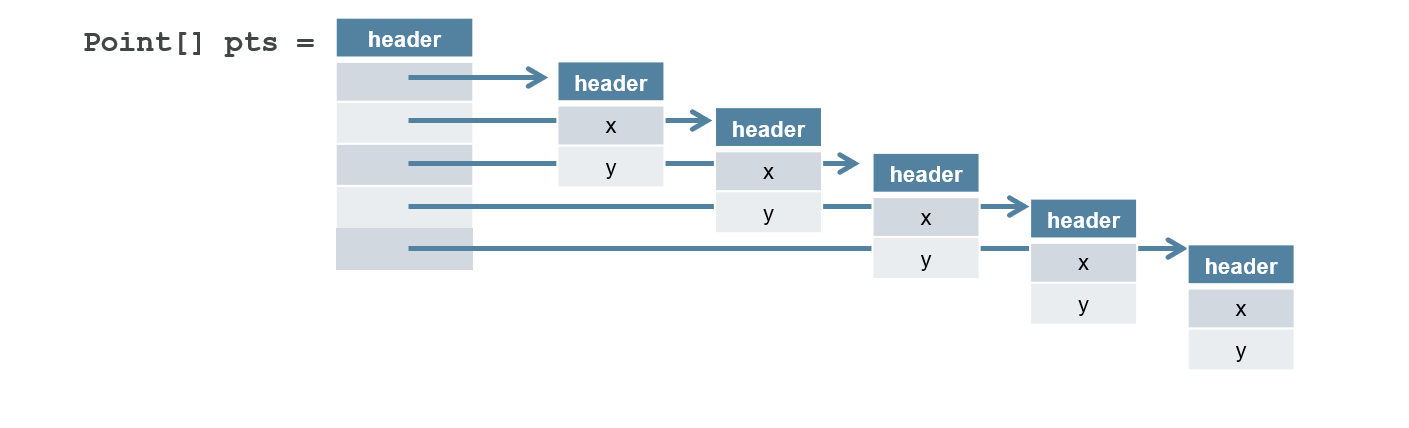
\includegraphics[width=0.95\linewidth]{image/reference.png}
\end{figure}
Класс Point содержит в себе два поля x, y типа int. Как описывалось ранее, Java работает с 
такого рода объектами как со ссылками. Потому массив "pts" содержит в себе указатели. В таком случае при доступе к полю "x" элемента i требуется дополнительное разыменования указателя, и только потом поступаемся по поля x.

\begin{lstlisting}
Point value = pts[i].x;
\end{lstlisting}
Однако в реальности мы имеем дополнительные издержки, связанные с исполнением load барьера и проверкой прочитанного значения на null:
\begin{lstlisting}
Point* tmp = &pts[i];
Point actual_value = load-barrier(tmp);
if (actual_value == null) {
	throw new NullPointerException();
}
\end{lstlisting}
В итоге это приводит к довольно дорогостоящему доступу к элементу массива. Было бы полезно избавиться от дополнительных накладных расходов на доступ к полю. Одним из возможных способов является расположение всего под графа в виде линейного участка памяти, как указано на рисунке \ref{values-graph}.

\begin{figure}[h]
	\caption{Массив значений}\label{values-graph}
	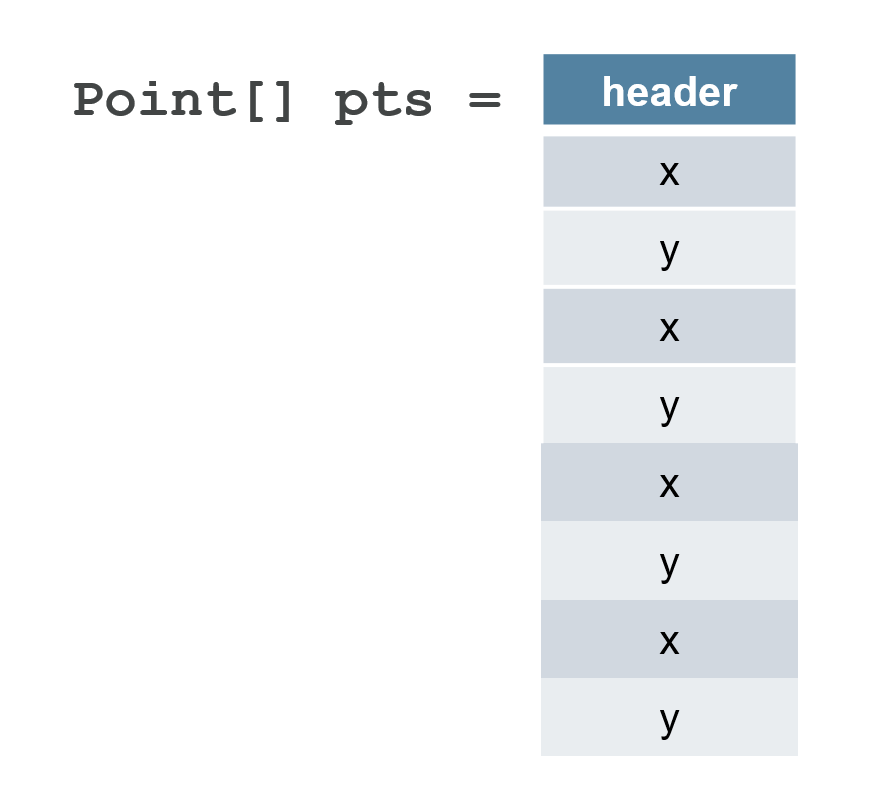
\includegraphics[width=0.65\linewidth]{image/flattened-points.png}
\end{figure}
По сравнению с предыдущей раскладкой объектов, у последней есть ряд преимуществ:
\begin{itemize}
	\item Улучшается локальность процессорного кеша. Поскольку объекты находятся рядом, а не разбросаны по всей куче, при чтении одного элемента в линейку кеша могут быть записаны соседние элементы. Это потенциально увеличивает производительность последовательного доступа к элементам массива.
	\item Load барьер и проверка на null не нужны. Адрес конкретного поля i-того элемента могут быть вычислены с помощью адресной арифметики. И поскольку виртуальная машина подразумевает, что в таком массиве не бывает null значений, проверки на null исчезают.
	\item Последовательный доступ к элементам может быть автоматически векторизован компилятором
\end{itemize}
К сожалению на данный момент JVM и язык Java не поддерживают возможность создания такого рода структуры данных. Данная работа посвящена ее разработке. Для этого были поставлены следующие задачи: 
\begin{enumerate}
	\item Изучить похожие работы
	\item Реализация данной структуры данных. Она подразумевает разработку удобного интерфейса, поддержку на уровне среды исполнения
	\item Измерить производительность и проанализировать результаты
	\item Найти и по возможности применить данную структуру данных для реализации других. Так же провести тестирование производительности
	\item Подготовить документацию  
\end{enumerate}
Данная работа проводилась на базе виртуальной машины Zing, разрабатываемой Azul Systems. Ее более подробное описание можно найти в секции \ref{Java}

\clearpage